\chapter{Striatum and Effort} \label{ch:lesion}
In the last chapter, I presented many experiments, all in support of the hypothesis that time estimation is embodied and that accurate timing requires stereotyped interaction with the environment.
Stereotyped interactions appear as motor routines to the external observer, e.g., the superstitious behavior of pigeons (\autoref{ch:intro:EmbodiedClock}) and the wait-and-run routine of rats (\autoref{ch:time}).
Thus, the question of how the brain measures the elapsed time is translated to how the brain generates or controls motor routines.
In this study, we focused on the striatum, the main input nuclei of the \gls{bg}, since its motor-related functions are long-reported, well-known, and still debated.\footnotemark\
We took advantage of the motor routine developed by the animals in the treadmill task, i.e., the wait-and-run motor routine (\Autoref{fig:time:CtrlTrd}{d}) to investigate the role of the striatum in performing and controlling the kinematics of motor routines.

\footnotetext{
    The materials related to striatal function in this document were largely borrowed from~\cite{JuradoParras2020}.
}
To obtain a drop of sweetened water, rats had to wait for a fixed \gls{gt} of 7~s from trial onset before entering the reward area located at the front of the treadmill, while the belt was slowly moving backward (\Autoref{fig:lesion:task}{A}).
Across training sessions composed of $\sim$120~trials, animals learned to wait longer and longer to enter the reward are just after the \gls{gt} and achieve higher percentage of correct trials (\Autoref{fig:lesion:task}{B}, and \autoref{fig:appendix:CorrectTrialCurve}).
Task proficiency was clearly associated with the acquisition and reliable performance of the following routine (\Autoref{fig:lesion:task}{C}):
\begin{enumerate}[noitemsep]
    \item during the intertrial, following the consumption of the reward, rats remained in the reward area;
    \item when the treadmill was turned on (trial onset), they did not move and let the belt carry them away from the reward area;
    \item when they reached the rear wall of the treadmill, they started outrunning the treadmill to reenter the reward area, i.e., the \gls{et} just after 7~s ($ET\geq GT$).
\end{enumerate}
After 2--3 weeks of daily practice, rats used this wait-and-run routine in about 75\% of the trials (\Autoref{fig:lesion:task}{C}, see \autoref{ch:methods:dataAnalysis} for the operational definition of this routine).
Finally, learning this routine was paralleled by a robust invigoration of the running phase of the motor routine toward the reward area (\Autoref{fig:lesion:task}{D}).

\section{Striatal Lesion}
\label{ch:lesion:lesion}
\begin{figure}[bt!]
	\begin{center}
		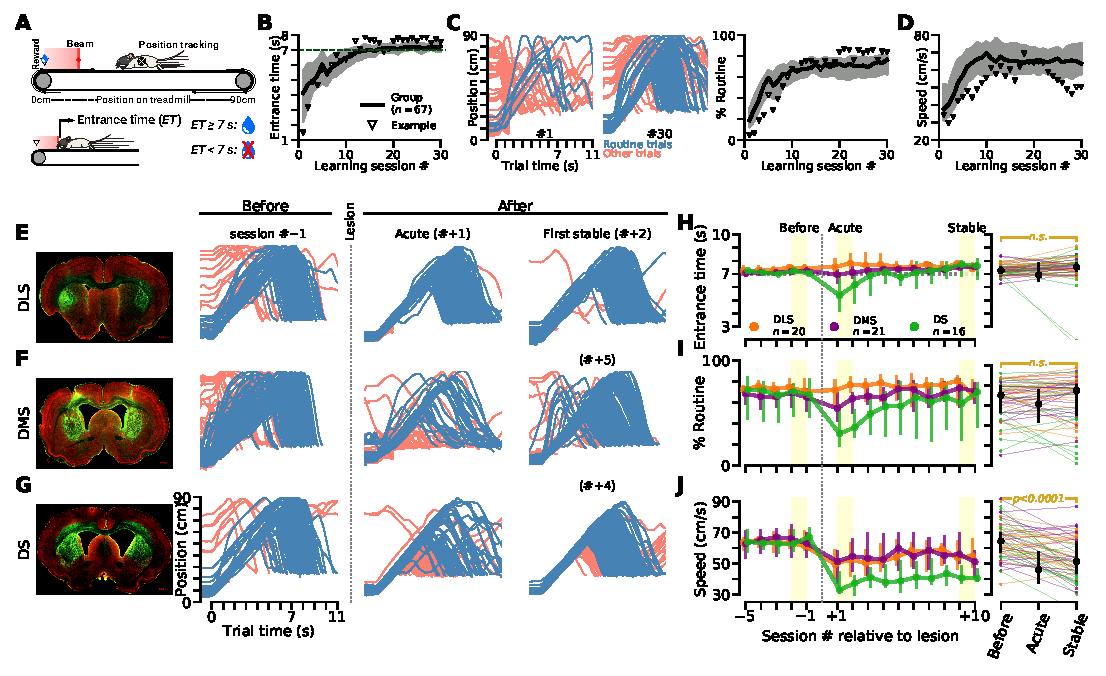
\includegraphics[width=\textwidth]{ch-lesion/figures/Task_Example_Group.pdf}
		\caption[The Striatum Energizes Motor Routines]
		{\textbf{The dorsal striatum is necessary to invigorate the running component of a motor routine.}
		\textbf{A)}
		Experimental apparatus and task rules, also refer to \autoref{fig:methods:taskRules}.
		\textbf{B)}
		Median \gls{et} across training sessions for all the rats trained in this task.
		Shaded area represents the 25th and 75th percentiles.
		Triangular markers in panels~B to~D indicate the performance for the example animal whose trajectories are shown in panel~C, left.
		\textbf{C)}
		Trajectories of an example animal on the treadmill, for all the trials performed in sessions \#1 and \#30 (\textit{left}).
		Percentage of trials during which animals performed the wait-and-run routine, across training sessions (\textit{right}).
		\textbf{D)}
		The running speed with which animals ran toward the reward area, across training sessions.
		\textbf{E-G)}
		Histology (\textit{left}, GFAP in green shows gliosis, red is NeuN) and trajectories of single animals with bilateral lesions of the striatum (\textit{right}) in sessions before and after the lesion.
		`\#'~indicates session number relative to the lesion operation.
		\textbf{H-J)}
		\textit{Left}: time course of the lesion effect on behavioral measures.
		\textit{Right}: statistical comparison of the group data before vs.\ (long) after the lesion (10000 resamples).
		Trajectory plots in panels~C, and~E--G are cut at the \gls{et}.
		}
		\label{fig:lesion:task}
	\end{center}
\end{figure}
\par
Once the performance was stable, after at least 30 training sessions, we performed fiber-sparing lesions of the striatum ($n=57$ animals, for the lesion protocol, see \autoref{ch:method:lesion}).
The lesions targeted either the \gls{dls} or the \gls{dms}, or both territories, the entire \gls{ds} (\Autoref{fig:lesion:task}{E-G}, see also \autoref{fig:method:LesionSizeLocation}).
Behavioral testing resumed two weeks after the lesion surgery.
Visually, the animals had normal behavior (locomotion, food/water intake) in their homecage at the end of the recovery period.
\par
After the lesion, the behavior of the animals could be divided into an `acute' phase in the first few sessions post-lesion, and a `stable' phase that begins $\sim$9 sessions after the lesion and persists.
This dichotomy does not apply to every animal, apparently animals with bigger lesions have a stronger acute effect.
This can be seen in example animals of \Autoref{fig:lesion:task}{F,~G}, and at the population level in \Autoref{fig:lesion:task}{H}, however, the case illustrated in \Autoref{fig:lesion:task}{E} is an example of a rat with smaller lesion and no acute condition.
To better visualize the acute effect, I grouped the first two post-lesion sessions and presented their average statistics throughout this manuscript.
Similarly, sessions $+9$ and $+10$ were also grouped to represent the stable effect of the lesion.
Animals with this acute effect ran toward the reward area prematurely after trial onset and, consequently, a drop in the usage of the wait-and-run routine was observed during these first post-lesion sessions (\Autoref{fig:lesion:task}{I}).
Surprisingly, most of these animals recovered from this initial impairment and after a few additional sessions, task proficiency was similar to the pre-lesion level (\Autoref{fig:lesion:task}{H-I}, right panels, compare the stable condition to the `before' condition).
Moreover, for most of the animals with a lesion restricted to the DLS and DMS, task proficiency was virtually unaltered when resuming behavioral testing.
We then looked at animals' speed, the velocity with which they outran the opposing treadmill in the third step of the wait-and-run motor routine (see \autoref{ch:methods:dataAnalysis} for the definition).
Strikingly, the animals' speed was irreversibly reduced following striatal lesion (\Autoref{fig:lesion:task}{I}).
In addition, the difference in speed due to lesion was strongly correlated with the size of the lesion (\Autoref{fig:appendix:spd}{A}).
\begin{figure}[tb!]
    \begin{center}
        \includegraphics[width=\textwidth]{ch-lesion/figures/Lick.pdf}
        \caption[Licking Behavior After Striatal Lesion]
        {\textbf{Licking behavior mostly unaffected by the striatal lesion.}
        \textbf{A)}
        Trial-by-trial licking pattern (\textit{top}) and averaged lick rate aligned to intertrial onset for a single animal in 3~sessions (1~just before and 2~after lesion).
        Each tick shows one lick in the reward delivery port.
        \textbf{B-D)}
        Effect of striatal lesion on lick onset delay (\textit{B}), number of licks per intertrial (\textit{C}) and peak licking frequency (\textit{D}).
        Same color code for individual lesion type as in \autoref{fig:lesion:task}.
        }
        \label{fig:lesion:lick}
    \end{center}
\end{figure}
Moreover, the maintained task proficiency following striatal lesion suggested that the motivation of the animals to perform the task and to obtain rewards was preserved.
In agreement with this statement, animals with a striatal lesion kept licking the reward after committing correct trials(\Autoref{fig:lesion:lick}{A}).
They licked the number of times after reward delivery and also their peak lick frequency was not affected (\Autoref{fig:lesion:lick}{C-D}).
However, they systematically started to lick later (\Autoref{fig:lesion:lick}{B}).
Much like the speed, this effect was also irreversible, and might be a measure of slower speed in approaching the reward port after crossing the infrared beam (which is $\sim$10~cm from the reward port), or slower postural adjustments to consume the delivered reward.
Thus far, these results suggest that the striatum is selectively critical for the invigoration of the reward-oriented active component of the wait-and-run routine.


\section{Reverse Treadmill Task}
\label{ch:lesion:rev}

What was the reason for the acute effect right after the break?
At this stage, we can not rule out that the transient impairment in performance induced by large striatal lesions reflects deterioration of the motor routine and reversal to the behavior expressed before routine acquisition, i.e., staying in the front, possibly to get the reward (see \Autoref{fig:time:CtrlTrd}{e} and \autoref{fig:appendix:initPos}).
This impairment then could have been compensated in subsequent post-lesion sessions through a striatum-independent learning process.
To test this hypothesis we modified the task such that the treadmill belt moved slowly toward the reward area, instead of away from it.
This configuration, hereafter called the `reverse' treadmill, allows the animals to locomote to the back of the treadmill during the intertrial while the treadmill is not moving, stay still upon trial onset and be passively transported to the reward port at the right time ($ET>GT$).
Such a ``run-and-wait'' motor routine is qualitatively comparable to the original run-and-wait routine, and critically, initiates in the back of the treadmill, hence we can dissociate routine initiation from reversal to the behavior expressed before routine acquisition.
Another group of animals were trained in this version of the task and learned to proficiently perform the task by adopting the run-and-wait routine described above (\Autoref{fig:lesion:rev}{A}).
That is, after extensive training, animals were in the back of the treadmill at trial onset in a bigger fraction of the trials. 
\begin{figure}[bt!]
	\begin{center}
		\includegraphics[width=\textwidth]{ch-lesion/figures/ReverseTreadmill.pdf}
		\caption[Preserved Motor Routine Performance After Lesion]
		{\textbf{Striatal lesion spared the performance of a motor routine.}
		\textbf{A)}
		Trajectory of a proficient animal trained in a version of the treadmill task in which the belt moved toward the reward area (rather than away from it, see \autoref{ch:methods:rev}).
		9~consecutive trials (shaded areas) and intertrials (white areas) are shown.
		\textbf{B)}
		Trajectories from a single representative animal in two sessions before and two sessions after lesion.
		\textbf{C-D)}
		Comparison of \gls{et} (\textit{C}) and percentage of the ``run-and-wait'' (reverse) routine usage (\textit{D}), before and after \gls{dls} lesion.
		}
		\label{fig:lesion:rev}
	\end{center}
\end{figure}
If the striatal lesion abolished the ability to perform this motor routine, we expect animals to start the trials close to the reward area, at least in the first post-lesion sessions.
On the contrary, the performance of the run-and-wait routine was spared by striatal lesions (\Autoref{fig:lesion:rev}{C-D}).
It is noteworthy that lack of effect of the striatal lesion on the performance of the motor routine could be due to the fact that learning the reverse treadmill task was easier than the normal treadmill task, thus the relearning procedure might have happened during the very first session after the lesion.
This is unlikely to be the case since initial learning of the reverse treadmill task took a similar learning curve compared to that of the normal treadmill task (\autoref{fig:appendix:revLearn}).
Altogether, these results indicate that the striatum is not required to initiate or execute the sequential steps of the learned motor routine, but it is critical to invigorate its reward-oriented running phase.


\section{Intact Motor Function}
\label{ch:lesion:motorOk}

To better understand the origin of this vigor deficit, we examined whether striatal lesions affected elementary motor abilities of the animals.
First, we tested basic locomotor activity in a novel environment without any rewards.
We tracked their position during the first 10~min of exploration in a novel treadmill (without any food or water restriction prior to this test, see \autoref{ch:methods:loco} for more details).
Rats with \gls{dls} lesions had an identical amount of displacement on the treadmill compared to the control ones (\Autoref{fig:lesion:motorOk}{A}).
Thus, basic locomotion is spared by lesion of the striatum.
Then, we aimed to examine whether lesioned animals have the ability to outrun the treadmill, i.e., run faster than $\sim$10~cm/s.
We progressively increased the treadmill speed across 30~s long trials, interleaved by 30~s long intertrials.
Same groups of animals as in the last test ($n=12$ rats) performed similarly in this free running task (\Autoref{fig:lesion:motorOk}{B}).
Therefore, lesioned animals are able to run at speeds much faster than 10~cm/s if they are forced to.
Of note, the average speed of animals with a striatal lesion during the trials was similar to normal rats, but only for slower treadmill speeds.
\begin{figure}[bth!]
 \begin{center}
	\includegraphics[scale=1]{ch-lesion/figures/MotorPreserved.pdf}
	\caption[Preserved Motor Control After Striatal Lesion]
	{\textbf{Preserved modulation of running speed and spontaneous locomotor activity following striatal lesion.}
	\textbf{(A)} Average speed when rats ran toward the reward area. Data were split according to the position of the rats on the treadmill when initiating their runs.
	\textbf{(B)} Speed of runs initiated either in the back or the middle portion of the treadmill calculated for each animal on the last 5 sessions before lesion (left) and sessions \#4 to \#9 after lesion (right).
	\textbf{(C)} Distance ran while exploring a new immobile treadmill for non-lesioned and lesioned rats ($n=12$).
	\textbf{(D)} Average running speed in a free running task (no reward) in which control and lesioned rats were submitted to trials with incremental treadmill speed (same color code as in C).
	Horizontal golden lines indicated significant differences between groups.
	}
	\label{fig:lesion:motorOk}
 \end{center}
\end{figure}
In trials in which the treadmill moved faster than 20~cm/s, even though lesioned rats managed to keep running, their speed had the tendency to be marginally slower than control animals.
This effect mimics the overall tendency of the animals to `choose' a slower pace, be it in approaching the reward area or starting to lick the available reward.
Next, we dived into the speed profile of the animals to investigate the essential ability of modulating the running speed.
We compared their running speed in trials in which the running epoch was initiated from the rear portion of the treadmill, versus the middle of the treadmill (in \Autoref{fig:lesion:motorOk}{C}: Back vs. Mid).
Non-lesioned animals ran faster when they initiated their runs from the back of the treadmill (\Autoref{fig:lesion:motorOk}{D}).
Interestingly, this modulation, too, was maintained after striatal lesions, although running speeds were generally slower following the lesion.


\section{Effort, The Underlying Mechanism}
\label{ch:lesion:effort}
\begin{figure}[bth!]
	\begin{center}
		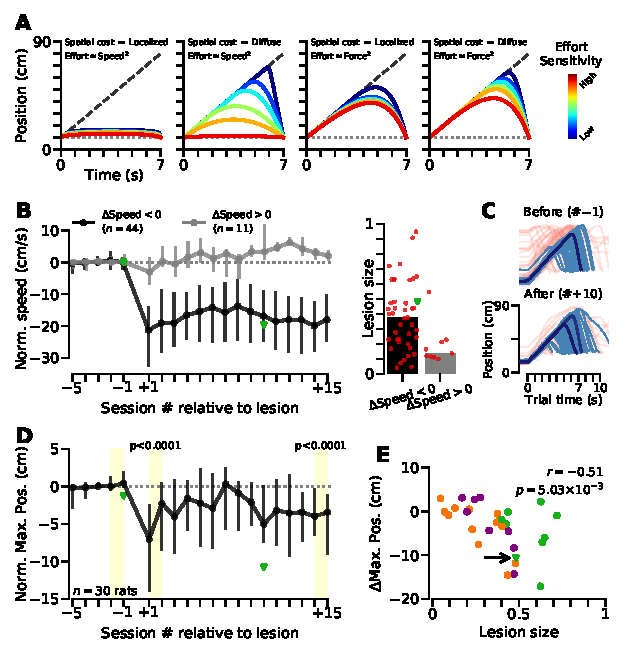
\includegraphics[scale=1]{ch-lesion/figures/MaxPosAnalysis.pdf}
		\caption[Optimal Trajectory and Experimental Validation]
		{\textbf{Optimal trajectory vs effort sensibility and experimental validation.}
		\textbf{A)} Optimal trajectories predicted by models with different effort and spatial costs approximations.
		The cost of premature entrance in the reward area (spatial cost) was simulated using a Heaviside function that was either localized ($\sim$step function with non-zero value within the reward area) or diffuse ($\sim$a sigmoid function whose value gradually decreases toward zero away from the reward area).
		Effort was approximated as the square value of either the muscular force produced by the animals or of its speed.
		\textbf{B)} \textit{Left}, animals were divided into two groups based on the significance of the dS lesion effect on running speed.
		\textit{Right}, lesion size for animals in those two groups.
		\textbf{C)} Effect of striatal lesion on the trajectories of a single animal.
		Only trials in which the routine was executed (thin blue lines) were taken into account to compute the median trajectory (bold blue line).
		\textbf{D)} Effect of striatal lesion on the maximum position of the median trajectory across routine trials.
		\textbf{E)} Effect of striatal lesion on the maximum position versus lesion size.
		Same color code for individual lesion type as in \autoref{fig:lesion:task}.
		Green triangles in panels~B,~D, and~E are data points from the example animal whose trajectories, before and after lesion, are shown in panel~C.
		}
		\label{fig:lesion:maxPos}
	\end{center}
\end{figure}
Since the striatal lesion spared the rats' ability to modulate their running speed, the most parsimonious account of our results is that lesioned animals `preferred' slower speeds.
We took advantage of the optimal control framework that relies on the assumption that animal behavior is optimal with respect to a cost function.
A simple model was implemented to simulate the optimal trajectory taking into account costs related to energy expenditure (effort) and those imposed by the task rules (running in the front is costly as it leads to premature \gls{et}, which is punished).
Four cost functions were used to model speed/force-based effort, and localized/diffuse penalty related to staying in the front of the treadmill (see \cite{JuradoParras2020} for more details).
We found that higher effort sensitivity, regardless of exact cost function parameters, resulted in optimal trajectories with smaller `maximum position', i.e., earlier run-phase initiation (\Autoref{fig:lesion:maxPos}{A}).
Hence, combination of late initiation of the run-phase together with fast running speeds was not used.
This result is not only in agreement with the reduced running speed observed following the lesion, but is also reminiscent of the behavior observed during the very first post-lesion sessions, when animals with larger \gls{ds} lesions ran mainly close to the reward area (\Autoref{fig:lesion:task}{F,~G}). 
We thus reanalyzed the effect of striatal lesion on the trajectory, focusing on animals with a significant reduction in running speed (\Autoref{fig:lesion:maxPos}{B}).
We also limited the analysis to trials during which animals perfectly executed the wait-and-run routine, since those are the trials for which defining the maximum position is relevant.
Strikingly, following striatal lesions of various sizes and locations, rats started running forward earlier relative the length of the treadmill, i.e., a smaller maximum position (\Autoref{fig:lesion:maxPos}{D}).
This effect too, similar to speed, persisted after three weeks of daily sessions post-lesion.
Also, the reduction in maximum position was well-correlated with lesion size, the bigger the lesion, the bigger the reduction (\Autoref{fig:lesion:maxPos}{E}).


\section[Preserved Routine Learning]{(Mostly) Preserved Routine Learning}
\label{ch:lesion:learn}
Our results indicate that the \gls{ds} is not required for the execution of motor routines (at least those similar to the wait-and-run), rather it is influencing kinematics of learned behaviors.
Performing striatal lesion prior to learning the task, i.e., in na\"{i}ve animals, further confirmed earlier results.
We found that striatal lesions performed in na\"{i}ve rats did not compromise their ability to learn the wait-and-run routine (\Autoref{fig:lesion:EarlyLesionLearning}{A}).
Both groups of animals, with lesion in either \gls{dls} or \gls{dms}, learned the task with similar profile to control (non-lesioned) rats.
Those animals with lesion in the entire \gls{ds}, however, showed a different trait.
A few of them with relatively larger lesion, failed to display performance improvement (\Autoref{fig:lesion:EarlyLesionLearning}{A}).
All of these animals ran most of the time in the front region of the treadmill (\Autoref{fig:lesion:EarlyLesionLearning}{B,~C}).
The rest of this group, similar to the \gls{dls} and \gls{dms} groups, eventually improved their performance.
In animals with striatal lesion performed before training, a robust reduction of running speed was also observed, an effect that was correlated with lesion size as well (\Autoref{fig:appendix:spd}{B}).
\begin{figure}[bth]
  \begin{center}
	\includegraphics[width=1\linewidth]{ch-lesion/figures/EarlyLesionLearning.pdf}
	\caption
	{\textbf{Effect of DLS, DMS and DS lesions performed before training on task learning.}
	Session-by-session change in performance (ET, upper panels; Percentage of trials in which the routine was used, lower panels) for animals without lesion (Control, left) and for animals that received a lesion before training (DLS, DMS, DS from left to right). 
	Thick black lines show indicate group average.
    Thin colorful lines indicate single animals.
    Thick gray lines in 3 rightmost columns indicate control performance for comparison.
    Horizontal golden lines indicate significant differences between control and lesion groups. 
	}
	\label{fig:lesion:EarlyLesionLearning}
  \end{center}
\end{figure}